% Figure 1 -- PlanGrad-UAV framework (Nature/TRC style, vector TikZ)
% Every symbol traced to Draft_v10.tex. No invented notation.
\documentclass[border=5pt]{standalone}
\usepackage[utf8]{inputenc}
\usepackage{amsmath,amssymb,bm}
\usepackage{tikz}
\usepackage{helvet}
\renewcommand{\familydefault}{\sfdefault}
\usetikzlibrary{arrows.meta,positioning,calc,decorations.pathmorphing,patterns}

\newcommand{\bx}{\bm{x}}   % Draft_v10.tex:52
\newcommand{\bu}{\bm{u}}   % Draft_v10.tex:53

\definecolor{cPred}{HTML}{2F6F9F}
\definecolor{cPlan}{HTML}{1F7A63}
\definecolor{cDyn}{HTML}{B4622B}
\definecolor{cOut}{HTML}{5B5570}
\definecolor{cCal}{HTML}{7A7F87}
\definecolor{cGrad}{HTML}{A03028}
\definecolor{cInk}{HTML}{23262B}
\definecolor{cRule}{HTML}{9AA0A8}
\definecolor{cEgo}{HTML}{1B4F72}
\definecolor{cNb}{HTML}{C0721F}

\begin{document}
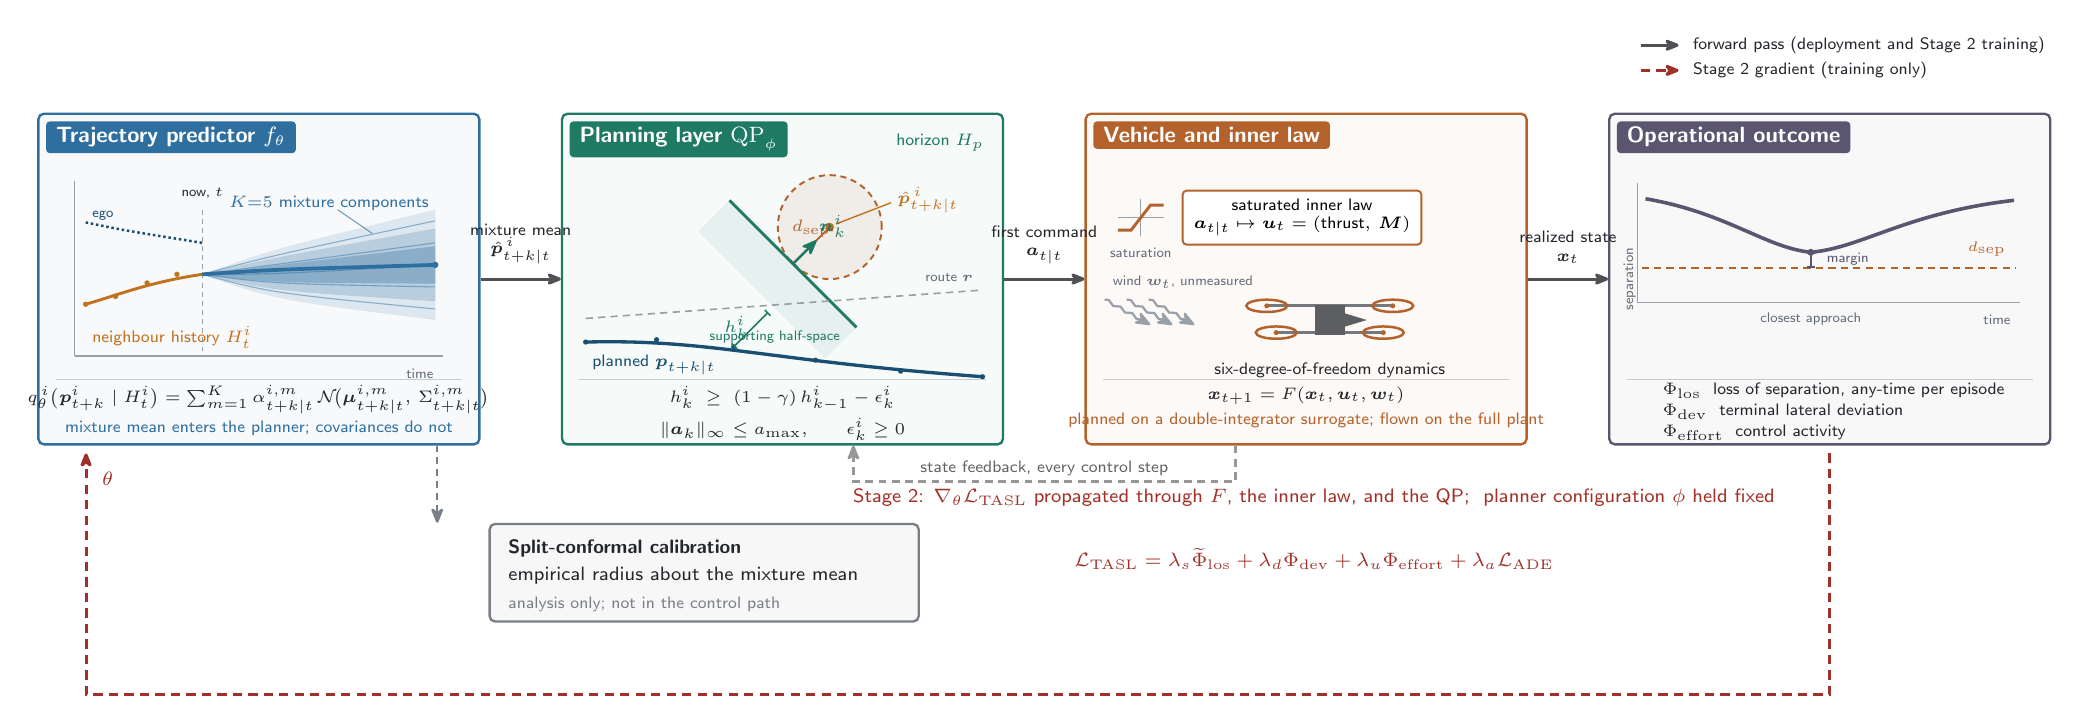
\begin{tikzpicture}[
  font=\sffamily,
  >={Stealth[round,length=2.4mm,width=1.9mm]},
  panel/.style={rounded corners=2pt,draw=#1,line width=.85pt,fill=#1!4},
  tag/.style={font=\sffamily\bfseries\fontsize{7.6}{8.6}\selectfont,
              text=white,fill=#1,inner xsep=3.6pt,inner ysep=2.2pt,
              rounded corners=1.4pt},
  eqs/.style={font=\fontsize{6.4}{7.6}\selectfont,text=cInk,inner sep=0pt},
  lab/.style={font=\sffamily\fontsize{6.5}{7.6}\selectfont,text=cInk},
  sml/.style={font=\sffamily\fontsize{6.0}{7.0}\selectfont,text=cInk},
  wee/.style={font=\sffamily\fontsize{5.4}{6.3}\selectfont,text=cRule!155},
  flow/.style={->,line width=1.1pt,draw=cInk!80},
  grad/.style={->,line width=1.1pt,draw=cGrad,dash pattern=on 3.4pt off 2.2pt},
]

% ===================== layout =====================
\def\W{5.60}\def\H{4.20}\def\G{1.05}
\def\hw{2.80}\def\hh{2.10}
\def\eqY{-1.60}

\coordinate (A) at (0,0);
\coordinate (B) at (\W+\G,0);
\coordinate (C) at (2*\W+2*\G,0);
\coordinate (D) at (3*\W+3*\G,0);

\newcommand{\eqrule}{%
  \draw[cRule!55,line width=.4pt] (-\hw+0.22,\eqY+0.32) -- (\hw-0.22,\eqY+0.32);}

% =====================================================================
% PANEL 1 -- Trajectory predictor
% =====================================================================
\begin{scope}[shift={(A)}]
  \node[panel=cPred,minimum width=\W cm,minimum height=\H cm] (P1) at (0,0) {};
  \node[tag=cPred,anchor=north west] at (-\hw+0.09,\hh-0.09)
       {Trajectory predictor $f_{\theta}$};
  \eqrule

  \def\ox{-2.34}\def\oy{-0.98}\def\pw{4.68}\def\ph{2.22}
  \draw[cRule,line width=.55pt] (\ox,\oy) -- (\ox+\pw,\oy);
  \draw[cRule,line width=.55pt] (\ox,\oy) -- (\ox,\oy+\ph);
  \node[wee,anchor=north east] at (\ox+\pw,\oy-0.04) {time};

  \def\nx{1.62}
  \draw[cRule,line width=.5pt,dash pattern=on 1.8pt off 1.5pt]
       (\ox+\nx,\oy+0.06) -- (\ox+\nx,\oy+\ph-0.34);
  \node[wee,anchor=south,text=cInk] at (\ox+\nx,\oy+\ph-0.34) {now, $t$};

  % neighbour observed history
  \draw[cNb,line width=1.05pt]
     (\ox+0.14,\oy+0.66) .. controls (\ox+0.56,\oy+0.78) and (\ox+0.94,\oy+0.94) ..
     (\ox+\nx,\oy+1.04);
  \foreach \t/\u in {0.14/0.66,0.52/0.76,0.92/0.93,1.30/1.04}
     \fill[cNb] (\ox+\t,\oy+\u) circle (0.034);
  \node[sml,anchor=west,text=cNb] at (\ox+0.10,\oy+0.24)
     {neighbour history $H^i_t$};

  % ego context track
  \draw[cEgo,line width=.9pt,densely dotted]
     (\ox+0.14,\oy+1.70) .. controls (\ox+0.62,\oy+1.60) .. (\ox+\nx,\oy+1.44);
  \node[wee,anchor=west,text=cEgo] at (\ox+0.10,\oy+1.78) {ego};

  % GMM fan
  \foreach \s/\op in {1.00/13, 0.66/21, 0.34/33}{
    \fill[cPred,opacity=\op/100]
      (\ox+\nx,\oy+1.04)
      .. controls (\ox+\nx+0.90,\oy+1.04+\s*0.32) ..
         (\ox+\pw-0.10,\oy+1.16+\s*0.70)
      -- (\ox+\pw-0.10,\oy+1.16-\s*0.70)
      .. controls (\ox+\nx+0.90,\oy+1.04-\s*0.32) ..
         (\ox+\nx,\oy+1.04) -- cycle;}
  \foreach \d in {-1,-0.5,0,0.5,1}{
    \draw[cPred,line width=.40pt,opacity=.48]
      (\ox+\nx,\oy+1.04) .. controls (\ox+\nx+0.90,\oy+1.04+\d*0.24) ..
      (\ox+\pw-0.10,\oy+1.16+\d*0.56);}
  \draw[cPred,line width=1.35pt]
      (\ox+\nx,\oy+1.04) .. controls (\ox+\nx+0.90,\oy+1.10) ..
      (\ox+\pw-0.10,\oy+1.16);
  \fill[cPred] (\ox+\pw-0.10,\oy+1.16) circle (0.040);
  \node[sml,anchor=east,text=cPred] (kl) at (\ox+\pw-0.06,\oy+1.94)
      {$K{=}5$ mixture components};
  \draw[cPred,line width=.4pt,opacity=.65]
      (\ox+\pw-1.34,\oy+1.86) -- (\ox+\pw-0.90,\oy+1.56);
\end{scope}
\node[eqs,anchor=north,align=center,
      font=\fontsize{6.1}{7.3}\selectfont] at ($(A)+(0,\eqY+0.26)$)
  {$q^{\,i}_{\theta}\big(\bm{p}^{i}_{t+k}\mid H^i_t\big)
    =\textstyle\sum_{m=1}^{K}\alpha^{i,m}_{t+k\mid t}\,
     \mathcal{N}\!\big(\bm{\mu}^{i,m}_{t+k\mid t},\,
     \Sigma^{i,m}_{t+k\mid t}\big)$\\[1.4pt]
   \footnotesize\sffamily\fontsize{5.6}{6.4}\selectfont
   \textcolor{cPred}{mixture mean enters the planner; covariances do not}};

% =====================================================================
% PANEL 2 -- Planning layer (CBF geometry)
% =====================================================================
\begin{scope}[shift={(B)}]
  \node[panel=cPlan,minimum width=\W cm,minimum height=\H cm] (P2) at (0,0) {};
  \node[tag=cPlan,anchor=north west] at (-\hw+0.09,\hh-0.09)
       {Planning layer $\mathrm{QP}_{\phi}$};
  \node[sml,anchor=north east,text=cPlan] at (\hw-0.12,\hh-0.13)
       {horizon $H_p$};
  \eqrule

  \coordinate (nb) at (0.60,0.66);
  \fill[cDyn,opacity=.085] (nb) circle (0.66);
  \draw[cDyn,line width=.7pt,dash pattern=on 2.2pt off 1.7pt] (nb) circle (0.66);
  \fill[cNb] (nb) circle (0.055);
  \node[sml,anchor=west,text=cNb,inner sep=1.6pt]
       at ($(nb)+(0.80,0.34)$) {$\hat{\bm{p}}^{\,i}_{t+k\mid t}$};
  \draw[cNb,line width=.5pt] ($(nb)+(0.08,0.04)$) -- ($(nb)+(0.78,0.31)$);

  \coordinate (tp) at ($(nb)+(225:0.66)$);
  \draw[cDyn,line width=.6pt,{Bar[width=1.2mm]}-{Bar[width=1.2mm]}] (nb) -- (tp);
  \node[sml,text=cDyn,anchor=south east,inner sep=1.2pt]
       at ($(nb)+(225:0.34)+(0.30,0.06)$) {$d_{\mathrm{sep}}$};

  \draw[cPlan,line width=1.0pt] ($(tp)+(135:1.14)$) -- ($(tp)+(-45:1.14)$);
  \fill[cPlan,opacity=.07]
       ($(tp)+(135:1.14)$) -- ($(tp)+(-45:1.14)$)
       -- ($(tp)+(-45:1.14)+(225:0.56)$) -- ($(tp)+(135:1.14)+(225:0.56)$) -- cycle;
  \draw[cPlan,line width=.85pt,->] (tp) -- ++(45:0.42);
  \node[sml,text=cPlan,anchor=south west,inner sep=.8pt]
       at ($(tp)+(45:0.42)$) {$\bm{n}^{i}_{k}$};
  \node[wee,anchor=north east,text=cPlan] at ($(tp)+(-45:1.02)$)
       {supporting half-space};

  \draw[cRule,line width=.6pt,dash pattern=on 2.6pt off 1.9pt]
       (-2.50,-0.50) -- (2.54,-0.14);
  \node[wee,anchor=south east] at (2.54,-0.16) {route $\bm{r}$};

  \draw[cEgo,line width=1.2pt]
       (-2.50,-0.80) .. controls (-0.90,-0.76) and (-0.20,-1.04) .. (2.54,-1.24);
  \foreach \t/\u in {-2.50/-0.80,-1.60/-0.77,-0.62/-0.86,0.42/-1.03,1.50/-1.17,2.54/-1.24}
       \fill[cEgo] (\t,\u) circle (0.033);
  \node[sml,anchor=north west,text=cEgo] at (-2.54,-0.84)
       {planned $\bm{p}_{t+k\mid t}$};

  \draw[cPlan,line width=.6pt,{Bar[width=1.0mm]}-{Bar[width=1.0mm]}]
       (-0.62,-0.86) -- ($(-0.62,-0.86)+(45:0.62)$);
  \node[sml,text=cPlan,anchor=north east,inner sep=1.2pt] at (-0.38,-0.42)
       {$h^{i}_{k}$};
\end{scope}
\node[eqs,anchor=north,align=center] at ($(B)+(0,\eqY+0.24)$)
  {$h^{i}_{k}\ \ge\ (1-\gamma)\,h^{i}_{k-1}-\epsilon^{i}_{k}$\\[1.6pt]
   $\|\bm{a}_k\|_{\infty}\le a_{\max},\qquad \epsilon^{i}_{k}\ge 0$};

% =====================================================================
% PANEL 3 -- Inner law + 6-DOF vehicle + wind
% =====================================================================
\begin{scope}[shift={(C)}]
  \node[panel=cDyn,minimum width=\W cm,minimum height=\H cm] (P3) at (0,0) {};
  \node[tag=cDyn,anchor=north west] at (-\hw+0.09,\hh-0.09)
       {Vehicle and inner law};
  \eqrule

  \begin{scope}[shift={(-2.10,0.78)},scale=0.44]
    \draw[cRule,line width=.5pt] (-0.66,0)--(0.66,0);
    \draw[cRule,line width=.5pt] (0,-0.54)--(0,0.54);
    \draw[cDyn,line width=1.05pt]
        (-0.66,-0.36)--(-0.28,-0.36)--(0.28,0.36)--(0.66,0.36);
  \end{scope}
  \node[wee,anchor=north] at (-2.10,0.52) {saturation};

  \node[draw=cDyn,fill=white,rounded corners=1.4pt,line width=.7pt,
        inner xsep=4pt,inner ysep=3pt,anchor=west,
        font=\sffamily\fontsize{6.2}{7.4}\selectfont,align=center]
       (IL) at (-1.58,0.78)
       {saturated inner law\\[-1pt]
        $\bm{a}_{t\mid t}\mapsto\bu_t=(\text{thrust},\,\bm{M})$};

  \begin{scope}[shift={(0.30,-0.52)}]
    \draw[cInk!62,line width=1.05pt] (-0.80,0.18)--(0.80,0.18);
    \draw[cInk!62,line width=1.05pt] (-0.68,-0.16)--(0.68,-0.16);
    \fill[cInk!74] (-0.19,-0.19) rectangle (0.19,0.19);
    \fill[cInk!74] (0.19,-0.085) -- (0.47,0) -- (0.19,0.085) -- cycle;
    \foreach \x/\y in {-0.80/0.18, 0.80/0.18, -0.68/-0.16, 0.68/-0.16}{
      \draw[cDyn,line width=.9pt] (\x,\y) ellipse (0.26 and 0.078);
      \fill[cDyn] (\x,\y) circle (0.032);}
  \end{scope}
  \node[sml,anchor=north] at (0.30,-0.94) {six-degree-of-freedom dynamics};

  \foreach \i in {0,1,2}{
    \draw[cRule,line width=.8pt,->,
          decorate,decoration={snake,amplitude=.55pt,segment length=4.8pt,
                               post length=2.5pt}]
      (-2.56+\i*0.28,-0.26) -- ++(0.58,-0.32);}
  \node[wee,anchor=west] at (-2.58,-0.04) {wind $\bm{w}_t$, unmeasured};
\end{scope}
\node[eqs,anchor=north,align=center] at ($(C)+(0,\eqY+0.24)$)
  {$\bx_{t+1}=F(\bx_t,\bu_t,\bm{w}_t)$\\[1.4pt]
   \sffamily\fontsize{5.6}{6.4}\selectfont
   \textcolor{cDyn}{planned on a double-integrator surrogate; flown on the full plant}};

% =====================================================================
% PANEL 4 -- Operational outcome
% =====================================================================
\begin{scope}[shift={(D)}]
  \node[panel=cOut,minimum width=\W cm,minimum height=\H cm] (P4) at (0,0) {};
  \node[tag=cOut,anchor=north west] at (-\hw+0.09,\hh-0.09)
       {Operational outcome};
  \eqrule

  \def\qx{-2.44}\def\qy{-0.30}\def\qw{4.86}\def\qh{1.52}
  \draw[cRule,line width=.55pt] (\qx,\qy) -- (\qx+\qw,\qy);
  \draw[cRule,line width=.55pt] (\qx,\qy) -- (\qx,\qy+\qh);
  \node[wee,anchor=north east] at (\qx+\qw,\qy-0.03) {time};
  \node[wee,rotate=90,anchor=south] at (\qx+0.10,\qy+0.30) {separation};

  \draw[cDyn,line width=.8pt,dash pattern=on 2.6pt off 1.9pt]
       (\qx+0.05,\qy+0.44) -- (\qx+\qw-0.05,\qy+0.44);
  \node[wee,anchor=south east,text=cDyn] at (\qx+\qw-0.06,\qy+0.46)
       {$d_{\mathrm{sep}}$};

  \draw[cOut,line width=1.3pt]
      (\qx+0.10,\qy+1.32)
      .. controls (\qx+1.14,\qy+1.14) and (\qx+1.62,\qy+0.70) ..
         (\qx+2.20,\qy+0.64)
      .. controls (\qx+2.86,\qy+0.70) and (\qx+3.40,\qy+1.14) ..
         (\qx+\qw-0.08,\qy+1.30);
  \fill[cOut] (\qx+2.20,\qy+0.64) circle (0.044);
  \draw[cOut,line width=.6pt,{Bar[width=1.0mm]}-{Bar[width=1.0mm]}]
       (\qx+2.20,\qy+0.44) -- (\qx+2.20,\qy+0.64);
  \node[wee,anchor=west,text=cOut] at (\qx+2.28,\qy+0.55) {margin};
  \node[wee,anchor=north,text=cRule!155] at (\qx+2.20,\qy-0.01)
       {closest approach};

  \node[anchor=north,align=left,
        font=\sffamily\fontsize{5.9}{7.0}\selectfont,text=cInk]
    at (0.05,\eqY+0.40)
    {$\Phi_{\mathrm{los}}$\ \ loss of separation, any-time per episode\\[0.6pt]
     $\Phi_{\mathrm{dev}}$\ \ terminal lateral deviation\\[0.6pt]
     $\Phi_{\mathrm{effort}}$\ \ control activity};
\end{scope}

% =====================================================================
% FORWARD FLOW
% =====================================================================
\draw[flow] (P1.east) -- (P2.west)
   node[lab,midway,above=1.6pt,align=center]
   {mixture mean\\[-1pt]$\hat{\bm{p}}^{\,i}_{t+k\mid t}$};
\draw[flow] (P2.east) -- (P3.west)
   node[lab,midway,above=1.6pt,align=center]
   {first command\\[-1pt]$\bm{a}_{t\mid t}$};
\draw[flow] (P3.east) -- (P4.west)
   node[lab,midway,above=1.6pt,align=center]
   {realized state\\[-1pt]$\bx_{t}$};

\draw[->,line width=.95pt,draw=cInk!48,dash pattern=on 2.8pt off 2.0pt]
   ($(P3.south)+(-0.9,0)$) -- ($(P3.south)+(-0.9,-0.46)$)
   -- node[sml,above,pos=0.5,text=cInk!72,inner sep=1.6pt]
      {state feedback, every control step}
      ($(P2.south)+(0.9,-0.46)$) -- ($(P2.south)+(0.9,0)$);

% =====================================================================
% CALIBRATION BRANCH
% =====================================================================
% calibration box sits right of the gradient riser, under panels 1-2
\node[draw=cCal,fill=cCal!6,rounded corners=2pt,line width=.85pt,
      minimum width=5.45cm,minimum height=1.24cm,anchor=north west]
     (CAL) at ($(P1.south east)+(0.10,-0.98)$) {};
\node[anchor=north west,align=left,
      font=\sffamily\fontsize{6.6}{8.2}\selectfont,text=cInk]
     at ($(CAL.north west)+(0.13,-0.10)$)
     {\textbf{Split-conformal calibration}\\[1.6pt]
      empirical radius about the mixture mean\\[1.6pt]
      \fontsize{5.8}{6.8}\selectfont
      \textcolor{cCal}{analysis only; not in the control path}};
\draw[->,line width=.9pt,draw=cCal,dash pattern=on 2.4pt off 1.9pt]
     ($(P1.south east)+(-0.55,0)$) -- ($(P1.south east)+(-0.55,-0.98)$);

% =====================================================================
% STAGE-2 GRADIENT RAIL -- below the calibration box
% =====================================================================
\def\gY{-3.16}
\draw[grad]
   ($(P4.south)+(0,-0.10)$) -- ($(P4.south)+(0,\gY)$)
   -- ($(P1.south west)+(0.62,\gY)$)
   -- ($(P1.south west)+(0.62,-0.10)$);
\node[anchor=south,align=center,
      font=\sffamily\fontsize{6.8}{8.2}\selectfont,text=cGrad]
   at ($(C)+(0.10,\gY+0.15)$)
   {Stage 2: $\nabla_{\theta}\mathcal{L}_{\mathrm{TASL}}$ propagated through
    $F$, the inner law, and the QP;\ \ planner configuration $\phi$ held fixed};
\node[anchor=north,font=\fontsize{6.6}{7.8}\selectfont,text=cGrad]
   at ($(C)+(0.10,\gY-0.13)$)
   {$\mathcal{L}_{\mathrm{TASL}}
     =\lambda_s\widetilde\Phi_{\mathrm{los}}
     +\lambda_d\Phi_{\mathrm{dev}}
     +\lambda_u\Phi_{\mathrm{effort}}
     +\lambda_a\mathcal{L}_{\mathrm{ADE}}$};
\node[anchor=west,font=\sffamily\fontsize{6.8}{7.8}\selectfont,text=cGrad]
   at ($(P1.south west)+(0.70,-0.42)$) {$\theta$};

% =====================================================================
% LEGEND
% =====================================================================
\begin{scope}[shift={($(D)+(\hw,\hh+0.68)$)}]
  \draw[flow] (-5.20,0.19) -- (-4.72,0.19);
  \node[lab,anchor=west] at (-4.66,0.19)
       {forward pass (deployment and Stage 2 training)};
  \draw[grad] (-5.20,-0.13) -- (-4.72,-0.13);
  \node[lab,anchor=west] at (-4.66,-0.13)
       {Stage 2 gradient (training only)};
\end{scope}

\end{tikzpicture}
\end{document}
